\chapter{Background and Related Work}
This chapter gives a detailed overview of the Bazo cryptocurrency and its underlying blockchain technology, as well as an introduction to existing applications and ones being developed at the same time as the blockchain explorer . Additionally it presents an analysis of existing blockchain explorers for two different cryptocurrencies, highlighting both similarities and differences in the implementation and functionality of the applications. The analysis plays a major role in the specification of the Bazo Blockchain Explorer, as it helps making design decisions for requirements.

\section{Bazo Blockchain and Cryptocurrency}
Developed in 2017 at the University of Zurich, the Bazo cryptocurrency is a private blockchain that aims to reduce administrative overhead, as well as extend the functionality of a financial service provider's bonus point reward system. Traditionally, for each merchant who wants to sell its products in the rewards shop of the service provider, specific contracts between the two parties need to be made. This makes expanding the bonus point system a time and resource consuming process. Bazo eliminates this restriction by introducing a cryptocurrency which allows to directly make transactions between merchants and users or even between users itself using Bazo Coins. The merchants itself do not need to form contracts with the service provider anymore, they can offer their products in exchange for Bazo Coins even at their own Point-of-Sale. The only interaction between the service provider and merchants consist of the exchange of Bazo Coins for fiat currency. A trial is planned, where the Bazo systems runs simultaneously to the existing bonus point system. Clients can request to exchange their current bonus points for Bazo Coins and vice-versa.

\subsection{Characteristics of Bazo}
Similarly to Ethereum \cite{ethereum}, Bazo uses an account-based model, which means that every user of the blockchain has a unique keypair (public and private key) that does not change after making a transaction. The public key acts as the address, when a user wants to receive funds from another user. The private key should only be held by its respective user and never leaves a user's device. It is used to sign transactions. A transaction only gets verified by the system if the correct private key has been used. In order to save bandwith, the blocks mined by the network do not contain all transaction data of transactions included in a block, only the hashes of transactions. The storage component of the Miner application saves all transaction data. There are 4 different types of transactions possible in the Bazo system.

\begin{itemize}
\item \textbf{Funds Transactions}
Funds Transactions are the most commonly used transactions, as they are the ones used by users of the blockchain to send Bazo Coins from one to another. Among other information, every transaction includes identifiers for the sender and receiver, and the amount of Bazo Coins being sent.
\item \textbf{Account Creation Transactions}
Only available to administrators of the system, Account Creation Transactions are used to generate new accounts. The public key of the new account is included int the transaction data, however the full keypair is stored on the device that generated the account.
\item \textbf{System Configuration Transactions}
Due to Bazo being a blockchain built from scratch, no guidelines for parameters such as the block interval or the minimum transaction exist. This is why these parameters can be changed on-the-fly by administrators using System Configuration Transactions.
\item \textbf{Stake Transactions}
\end{itemize}

Every transaction requires a fee to be processed. These fees are collected by the miners who successfully mine a block. This incentivises people to offer their processing power and in turn run the network. The administrator of Bazo will be the Financial Service Provider, meaning he alone has the power to add accounts and change system parameters.

\subsection{Bazo Applications}
In order for the Bazo system to be run, two command-line programs are needed. Both were developed as part of the original \emph{Bazo -- A Cryptocurrency from Scratch} \cite{bazo} thesis.

\begin{itemize}
\item \textbf{Bazo Miner}
This application, together with all other running Miners, makes up the network. It verifies transactions and mines blocks using a Proof-of-Work, or a Proof-of-Stake algorithm. On startup, the application copies the verified blockchain data, meaning the entire blockchain, from other miners into its storage component in order to be up-to-date and start verifying transactions. It also handles data concerning Bazo accounts and their balances, also known as the state of the blockchain.

\item \textbf{Bazo Client}
The Client is used for sending transactions to the network and making requests about the state. All types of transactions have to be made from the Client, including sending Configuration and Account Creation Transactions which are only reserved for administrators of the blockchain. A drawback of the Client application is the need to download the entire blockchain, similarly to the Miner in order for it to be useable.
\end{itemize}

Simultaneously to the development of the Bazo Blockchain Explorer, additional applications were developed, which enhance the scope and functionality of Bazo. 

\begin{itemize}
\item \textbf{Bazo Light Client \cite{marc}}
The Light Client fork of the Bazo Client application makes sending transactions possible, without having to download the entire blockchain. A Bloom Filter is responsible for only having to download blocks relevant to the user. Bandwidth and storage on the device can be saved with this Client implementation.
\item \textbf{Bazo Payment System \cite{payment}}
A web-based wallet and payment app have been developed, which enables users to manage their accounts and make transactions from their mobile devices or desktop computers, without having installed a native application. It also features Point-of Sale functionality, making the Bazo system useable in a real-life client-merchant situation.
\item \textbf{Bazo Interface \cite{marc}}
This interface is needed for both the Payment System and the blockchain explorer to send transactions to the network. Due to them not having implemented a Bazo Client, both applications are not able to build transactions on their own. This service receives the transaction information without the private key of the sender via a REST interface and responds with a transaction hash. This hash then gets signed with the private key stored on the device and sent back to the Interface for it to be broadcasted to the network.
\item \textbf{Proof-of-Stake Algorithm \cite{pos}}
\end{itemize}

\section{Blockchain Explorers and Analytics Platforms}
Since many cryptocurrencies are open-source and public \cite{ethereum} \cite{bitcoin}, often multiple blockchain explorers exist for a single currency. The most common application type for such explorers are web applications, publicly available and free to use on the internet. A blockchain explorer allows users to inspect blockchain data such as blocks and transactions, which may or may not be related to the user. A common use-case for block explorers are, after a user has submitted a transaction to the network, checking whether the user's transaction has been accepted or verified by the respective network. Some Cryptocurrency wallets, such as the Ledger Bitcoin Wallet \cite{btcwallet}, feature automatically generated links to blockchain explorers, so that a user can effortlessly check, whether his transaction has gone through or not. Other information blockchain users may find interesting, is statistical data about the network, such as 24 hour transaction volumes or market capitalization compared to other cryptocurrencies. 

\subsection{Blockexplorer.com \cite{blockexplorer}}
This blockchain explorer was built for both the Bitcoin \cite{bitcoin} and Bitcoin Cash \cite{bitcoincash} blockchains. The frontend of the web application is called Insight UI \cite{insightui} and is built using AngularJS \cite{angular}, a JavaScript \cite{javascript} framework. It interacts with the Insight API \cite{insightapi}, the corresponding backend. Insight API consists of a REST and websocket API for Bitcore Node \cite{bitcorenode}, a query and indexing service for the Bitcoin blockchain \cite{bitcoin}. The source code for both frontend and backend are available on GitHub \cite{insightui} \cite{insightapi}.

\begin{figure}
  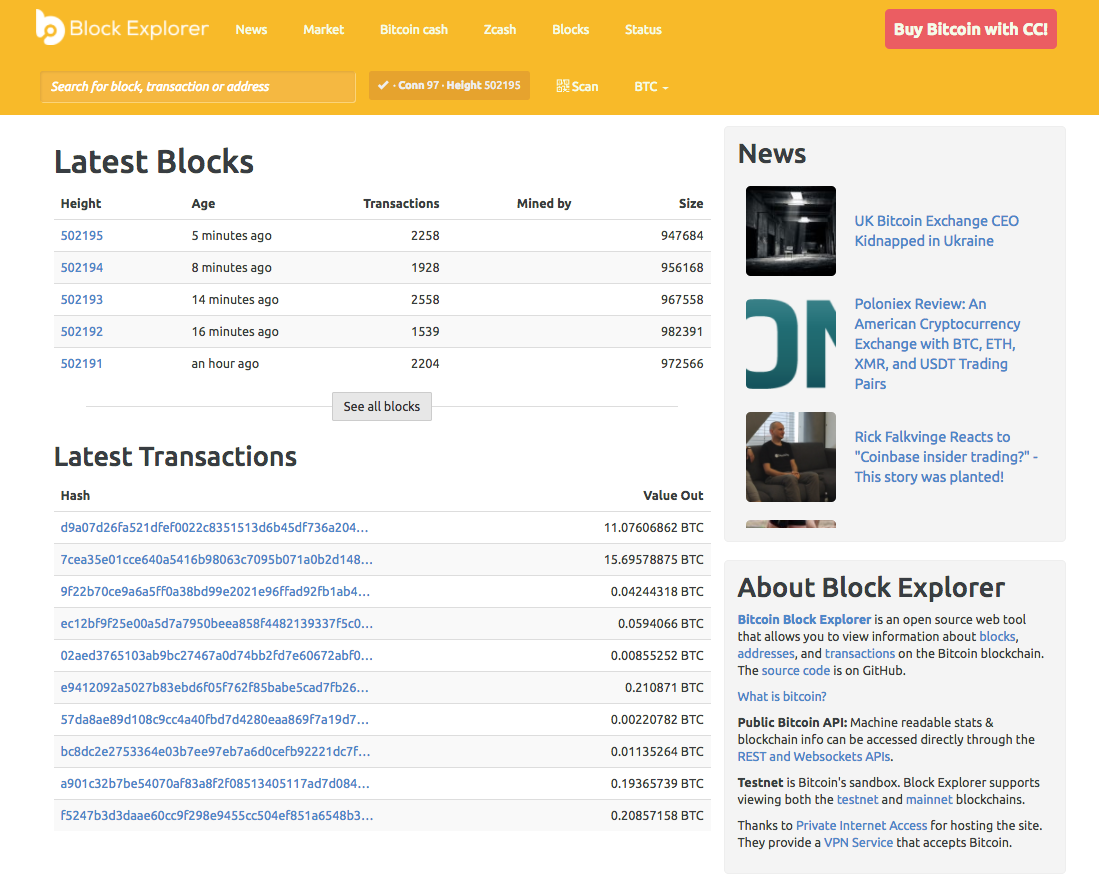
\includegraphics[width=\linewidth]{blockexplorer.png}
  \caption{Landing Page of blockexplorer.com \cite{blockexplorer}}
  \label{fig:blockexplorer1}
\end{figure}

\subsection{Etherscan.io \cite{etherscan}}
Etherscan is a blockchain explorer and statistics analysis platform for the Ethereum blockchain \cite{ethereum}. It uses Go Ethereum \cite{goethereum}, an implementation of the Ethereum protocol in the Go language \cite{golang}, in combination with Parity \cite{parity}, a client for interacting with the Ethereum blockchain \cite{ethereum}. Etherscan is a closed source project.

\begin{figure}
  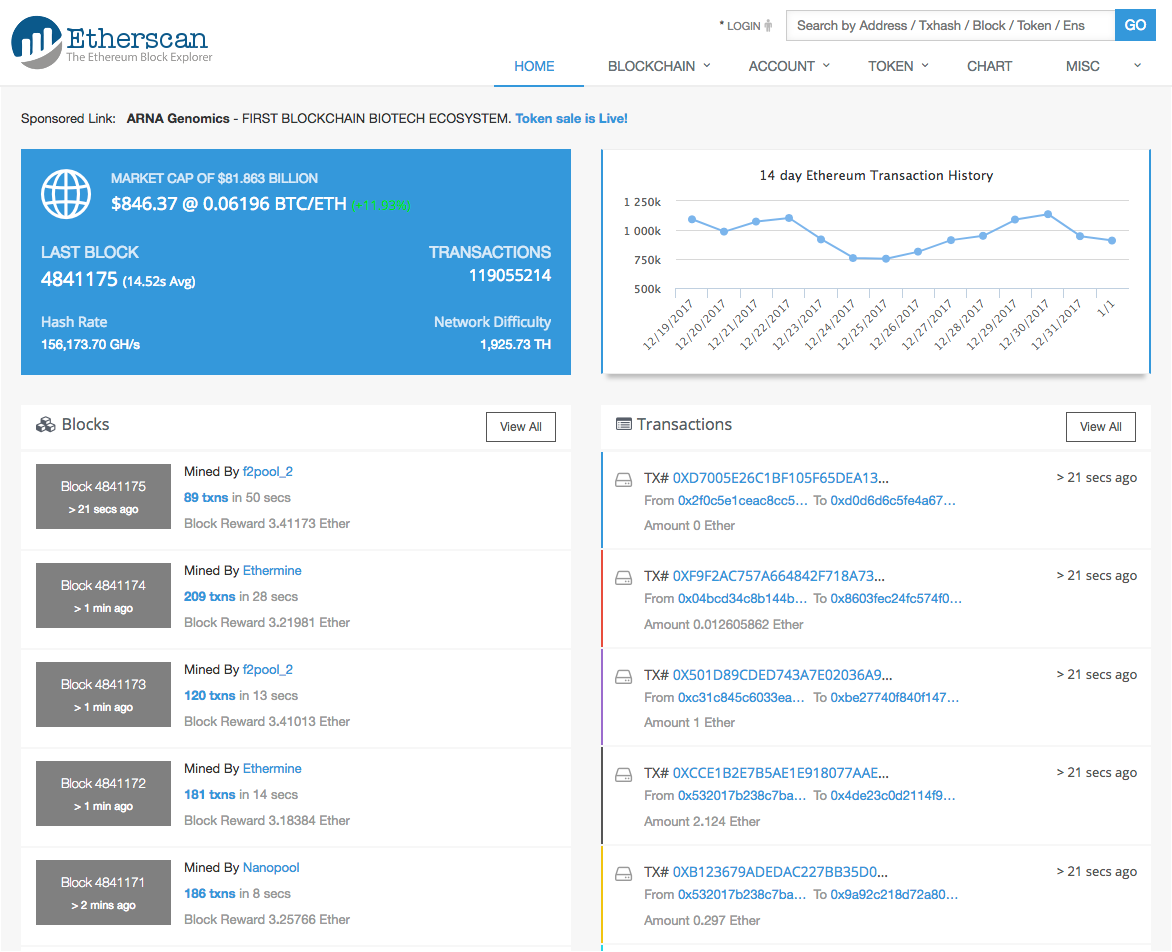
\includegraphics[width=\linewidth]{etherscan.png}
  \caption{Landing Page of etherscan.io \cite{etherscan}}
  \label{fig:etherscan1}
\end{figure}

\section{Analysis} \label{analysis}
Both explorers offer similar functionality as their core-feature: Structured views of blocks and transactions. The landing pages display the most recently mined blocks and transactions, with Blockexplorer offering real-time updates. Etherscan also displays statistical data about the chain, such as the market capitalization, mining difficulty and hash rate. A search feature is present on both sites, offering the user to search for transactions, blocks and accounts via their respective hashes. To browse the chain, links are used extensively (e.g. every block on the landing page links to its respective detailed block page). When presenting multiple objects on the same page, such as a list of blocks, the data is structured using tables. When multiple items are displayed using lists, less information about the items is given, compared to when a single item is viewed.

\subsection{Mutual Functions and Components}
DIFFERENE ETHEREUM BITCOIN
\begin{itemize}
\item \textbf{Landing Page}
Both explorers offer various information about their respective blockchain on the landing pages of the websites. The most recent blocks and transactions are displayed, with Etherscan using formatted list elements to differentiate between the individual blocks or transactions. Blockexplorer uses tables, that structures columns vertically. Among other, information regarding each block's age, height and number of transcations are featured. Etherscan displays more information regarding transactions, such as sender, receiver, compared to Blockexplorer, which only displays the transaction's hash and amount. Links to the full lists of blocks are present on both applications, however only Etherscan links to a full list of transactions.
\item \textbf{Blocks}
Lists, where all blocks ordered by age, are formatted using tables. More information about each block are displayed here, than on the landing page. Etherscan uses pagination to avoid having \emph{all} blocks displayed at once. Blockexplorer features a date-picker, that enables the display of only blocks that were mined on the chosen date. Both applications feature views for specific blocks, which display all information about a block. Links to other items like accounts and transactions are used heavily to make navigation of the page easier.
\item \textbf{Transactions}
As mentioned above, only Etherscan has a list displaying all transactions at once. It is structured using a table, similar to how blocks are structured on the page. Specific transactions can be viewed on both applications, however. Since Bitcoin uses a UTXO model \cite{bitcoin}, often not only one sender and one receiver are featured in a transaction, but multiple. This irregularity makes displaying senders and receivers in tables difficult and only possible on each transaction's detailed page on Blockexplorer.
\item \textbf{Accounts/Addresses}
Only Etherscan features a list of the most affluent accounts on the blockchain. On the detailed page for an account, both applications display all transactions where that account was either a sender or a receiver. The balance of each account or address is desplayed as well.
\item \textbf{Navbar and Search}
Both applications use a navbar, which is present on all pages. The navbar features links and dropdown menus to guide a user to the specific functions of the application. Etherscan has a significantly more extensive navbar than Blockexplorer, which makes an assessment ofthe overall funcitonality of Etherscan much easier. A search bar is also included in both navbars, where a user can search through blocks, transactions and addresses using hashes. The system does not require the user to choose emph{what} he is actually looking for, but finds that out automatically, given the hash a user enters is valid.
\item \textbf{Status}
\end{itemize}

\subsection{Functions and Components Specific to Blockexplorer.com}

\begin{itemize}
\item \textbf{Blockchain-Related News Feed}
A section displaying news, related to the blockchain community. 
\end{itemize}

\subsection{Functions and Components Specific to Etherscan.io}

\begin{itemize}
\item \textbf{Statistical Information}
Etherscan offers a vide variety of statistical information about the Ethereum network, displayed using graphs over time. A detailed overview of total Ether supply is also available.
\item \textbf{Calculation Tools}
A mining calculator is offered, that lets users evaluate the profitability of their mining operations. 
\end{itemize}

